% =====================================================================
%  Standalone TikZ source for the System Context diagram
%  Used to generate docs/requirements/diagrams/System-Context.png
%  Compile with: pdflatex system-context.tex
%  Then convert with: pdftoppm -r 200 -png system-context.pdf System-Context
% =====================================================================
\documentclass[border=10pt]{standalone}
\usepackage[T1]{fontenc}
\usepackage{lmodern}
\usepackage[dvipsnames]{xcolor}
\definecolor{primary}{HTML}{1F4E79}
\definecolor{accent}{HTML}{2E75B6}
\usepackage{tikz}
\usetikzlibrary{shapes.geometric, arrows.meta, positioning, fit, backgrounds, calc}

\begin{document}
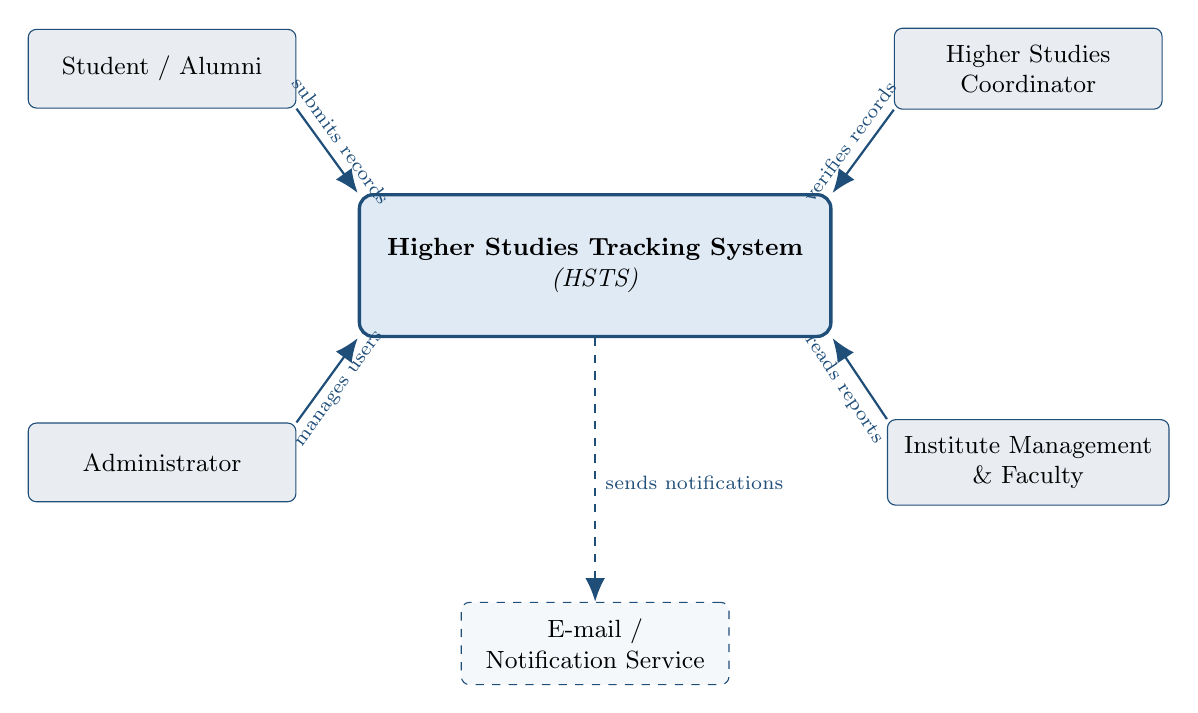
\begin{tikzpicture}[
    every node/.style={font=\small},
    actor/.style={
        rectangle, rounded corners=3pt,
        draw=primary, fill=primary!10,
        minimum width=3.4cm, minimum height=1cm,
        align=center, inner sep=6pt
    },
    system/.style={
        rectangle, rounded corners=5pt,
        draw=primary, very thick,
        fill=accent!15,
        minimum width=4.8cm, minimum height=1.8cm,
        align=center, inner sep=10pt
    },
    ext/.style={
        rectangle, rounded corners=3pt,
        draw=primary, fill=accent!5, dashed,
        minimum width=3.4cm, minimum height=1cm,
        align=center, inner sep=6pt
    },
    arrow/.style={-{Latex[length=3mm,width=2.5mm]}, thick, primary}
]
% System at the centre
\node[system] (sys) at (0, 0) {%
    \textbf{Higher Studies Tracking System}\\
    \textit{(HSTS)}
};

% Actors at the four corners around the system
\node[actor] (stu) at (-5.5, 2.5)  {Student / Alumni};
\node[actor] (coo) at ( 5.5, 2.5)  {Higher Studies\\Coordinator};
\node[actor] (adm) at (-5.5,-2.5) {Administrator};
\node[actor] (mgm) at ( 5.5,-2.5) {Institute Management\\ \& Faculty};

% External entity below the system
\node[ext]   (mail) at (0, -4.8) {E-mail /\\Notification Service};

% Arrows: each actor connects to the system
\draw[arrow] (stu.south east) -- node[above, sloped, font=\scriptsize]{submits records} (sys.north west);
\draw[arrow] (coo.south west) -- node[above, sloped, font=\scriptsize]{verifies records} (sys.north east);
\draw[arrow] (adm.north east) -- node[below, sloped, font=\scriptsize]{manages users} (sys.south west);
\draw[arrow] (mgm.north west) -- node[below, sloped, font=\scriptsize]{reads reports} (sys.south east);

% Arrow from system to external entity (vertical, no overlap with corner actors)
\draw[arrow, dashed] (sys.south) -- node[right, font=\scriptsize, pos=0.55]{sends notifications} (mail.north);
\end{tikzpicture}
\end{document}